% !TeX program = pdflatex
% !TeX root = ThreeDivergence.tex

\documentclass[../FeynCalcManual.tex]{subfiles}
\begin{document}
\hypertarget{threedivergence}{
\section{ThreeDivergence}\label{threedivergence}\index{ThreeDivergence}}

\texttt{ThreeDivergence[\allowbreak{}exp,\ \allowbreak{}CV[\allowbreak{}p,\ \allowbreak{}i]]}
calculates the partial derivative of \texttt{exp} w.r.t. \(p^i\).

\texttt{ThreeDivergence[\allowbreak{}exp,\ \allowbreak{}CV[\allowbreak{}p,\ \allowbreak{}i],\ \allowbreak{}CV[\allowbreak{}p,\ \allowbreak{}i],\ \allowbreak{}...]}
gives the multiple derivative.

Owing to the fact that in FeynCalc dummy Cartesian index are always
understood to be upper indices, applying \texttt{ThreeDivergence} to an
expression is equivalent to the action of
\(\nabla^i = \frac{\partial}{\partial p^i}\).

\subsection{See also}

\hyperlink{toc}{Overview}, \hyperlink{fourdivergence}{FourDivergence}.

\subsection{Examples}

\begin{Shaded}
\begin{Highlighting}[]
\NormalTok{CSP}\OperatorTok{[}\FunctionTok{p}\OperatorTok{,} \FunctionTok{q}\OperatorTok{]} 
 
\NormalTok{ThreeDivergence}\OperatorTok{[}\SpecialCharTok{\%}\OperatorTok{,}\NormalTok{ CV}\OperatorTok{[}\FunctionTok{q}\OperatorTok{,} \FunctionTok{i}\OperatorTok{]]}
\end{Highlighting}
\end{Shaded}

\begin{dmath*}\breakingcomma
\overline{p}\cdot \overline{q}
\end{dmath*}

\begin{dmath*}\breakingcomma
\overline{p}^i
\end{dmath*}

\begin{Shaded}
\begin{Highlighting}[]
\NormalTok{CSP}\OperatorTok{[}\FunctionTok{p} \SpecialCharTok{{-}} \FunctionTok{k}\OperatorTok{,} \FunctionTok{q}\OperatorTok{]} 
 
\NormalTok{ThreeDivergence}\OperatorTok{[}\SpecialCharTok{\%}\OperatorTok{,}\NormalTok{ CV}\OperatorTok{[}\FunctionTok{k}\OperatorTok{,} \FunctionTok{i}\OperatorTok{]]}
\end{Highlighting}
\end{Shaded}

\begin{dmath*}\breakingcomma
(\overline{p}-\overline{k})\cdot \overline{q}
\end{dmath*}

\begin{dmath*}\breakingcomma
-\overline{q}^i
\end{dmath*}

\begin{Shaded}
\begin{Highlighting}[]
\NormalTok{CFAD}\OperatorTok{[\{}\FunctionTok{p}\OperatorTok{,} \FunctionTok{m}\SpecialCharTok{\^{}}\DecValTok{2}\OperatorTok{\},} \FunctionTok{p} \SpecialCharTok{{-}} \FunctionTok{q}\OperatorTok{]} 
 
\NormalTok{ThreeDivergence}\OperatorTok{[}\SpecialCharTok{\%}\OperatorTok{,}\NormalTok{ CVD}\OperatorTok{[}\FunctionTok{p}\OperatorTok{,} \FunctionTok{i}\OperatorTok{]]}
\end{Highlighting}
\end{Shaded}

\begin{dmath*}\breakingcomma
\frac{1}{(p^2+m^2-i \eta ).((p-q)^2-i \eta )}
\end{dmath*}

\begin{dmath*}\breakingcomma
\frac{2 q^i-2 p^i}{(p^2+m^2-i \eta ).((p-q)^2-i \eta )^2}-\frac{2 p^i}{(p^2+m^2-i \eta )^2.((p-q)^2-i \eta )}
\end{dmath*}

Differentiation of \(3\)-vectors living in different dimensions (\(3\),
\(D-1\), \(D-4\)) works only in the t'Hooft-Veltman scheme

\begin{Shaded}
\begin{Highlighting}[]
\NormalTok{ThreeDivergence}\OperatorTok{[}\NormalTok{CVD}\OperatorTok{[}\FunctionTok{p}\OperatorTok{,} \FunctionTok{i}\OperatorTok{],}\NormalTok{ CV}\OperatorTok{[}\FunctionTok{p}\OperatorTok{,} \FunctionTok{j}\OperatorTok{]]}
\end{Highlighting}
\end{Shaded}

\FloatBarrier
\begin{figure}[!ht]
\centering
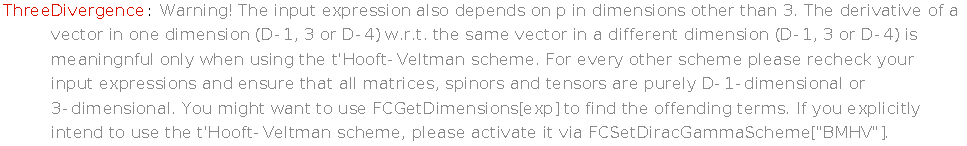
\includegraphics[width=0.6\linewidth]{img/1h9o7vmxcyb17.pdf}
\end{figure}
\FloatBarrier

\begin{dmath*}\breakingcomma
\text{\$Aborted}
\end{dmath*}

\begin{Shaded}
\begin{Highlighting}[]
\NormalTok{FCSetDiracGammaScheme}\OperatorTok{[}\StringTok{"BMHV"}\OperatorTok{]}\NormalTok{;}
\end{Highlighting}
\end{Shaded}

\begin{Shaded}
\begin{Highlighting}[]
\NormalTok{ThreeDivergence}\OperatorTok{[}\NormalTok{CVD}\OperatorTok{[}\FunctionTok{p}\OperatorTok{,} \FunctionTok{i}\OperatorTok{],}\NormalTok{ CV}\OperatorTok{[}\FunctionTok{p}\OperatorTok{,} \FunctionTok{j}\OperatorTok{]]}
\end{Highlighting}
\end{Shaded}

\begin{dmath*}\breakingcomma
\bar{\delta }^{ij}
\end{dmath*}
\end{document}
